\documentclass[10.5pt]{article}
\usepackage{amsmath,amssymb,amsthm}
\usepackage{listings}
\usepackage{graphicx}
\usepackage[shortlabels]{enumitem}
\usepackage{tikz}
\usepackage[margin=1in]{geometry}
\usepackage{fancyhdr}
\usepackage{epsfig} %% for loading postscript figures
\usepackage{amsmath}
\usepackage{float}
\usepackage{amssymb}
\usepackage{caption}
\usepackage{subfigure}
\usepackage{graphics}
\usepackage{titlesec}
\usepackage{mathrsfs}
\usepackage{amsfonts}
\usepackage{indentfirst}
\usepackage{fancybox}
\usepackage{tikz}

\renewcommand{\baselinestretch}{1.2}%Adjust Line Spacing
%\geometry{left=2.0cm,right=2.0cm,top=2.0cm,bottom=2.0cm}% Adjust Margins of the File
\usepackage{tikz-qtree}
\usetikzlibrary{graphs}
\tikzset{every tree node/.style={minimum width=2em,draw,circle},
	blank/.style={draw=none},
	edge from parent/.style=
	{draw,edge from parent path={(\tikzparentnode) -- (\tikzchildnode)}},
	level distance=1.2cm}
\setlength{\parindent}{0pt}
%\setlength{\parskip}{5pt plus 1pt}
\setlength{\headheight}{13.6pt}
\newcommand\question[2]{\vspace{.25in}\hrule\textbf{#1: #2}\vspace{.5em}\hrule\vspace{.10in}}
\renewcommand\part[1]{\vspace{.10in}\textbf{(#1)}}
\newcommand\algorithm{\vspace{.10in}\textbf{Algorithm: }}
\newcommand\correctness{\vspace{.10in}\textbf{Correctness: }}
\newcommand\runtime{\vspace{.10in}\textbf{Running time: }}
\pagestyle{fancyplain}
% Create horizontal rule command with an argument of height
\newcommand{\horrule}[1]{\rule{\linewidth}{#1}}
% Set the title here
\title{
	\normalfont \normalsize
	\textsc{ShanghaiTech University} \\ [25pt]
	\horrule{0.5pt} \\[0.4cm] % Thin top horizontal rule
	\huge CS101 Algorithms and Data Structures\\ % The assignment title
	\LARGE Fall 2019\\
	\LARGE Homework 3\\
	\horrule{2pt} \\[0.5cm] % Thick bottom horizontal rule
}
% wrong usage of \author, never mind
\author{}
\date{Due date: 23:59, October 6, 2019}

% set the header and footer
\pagestyle{fancy}
\lhead{CS101 Algorithms and Data Structures}
\chead{Homework 3}
\rhead{Due date: 23:59, October 6, 2019}
\cfoot{\thepage}
\renewcommand{\headrulewidth}{0.4pt}
\newtheorem{Q}{Question}
% special settings for the first page
\fancypagestyle{firstpage}
{
	\renewcommand{\headrulewidth}{0pt}
	\fancyhf{}
	\fancyfoot[C]{\thepage}
}

% Add the support for auto numbering
% use \problem{title} or \problem[number]{title} to add a new problem
% also \subproblem is supported, just use it like \subsection
\newcounter{ProblemCounter}
\newcounter{oldvalue}
\newcommand{\problem}[2][-1]{
	\setcounter{oldvalue}{\value{secnumdepth}}
	\setcounter{secnumdepth}{0}
	\ifnum#1>-1
	\setcounter{ProblemCounter}{0}
	\else
	\stepcounter{ProblemCounter}
	\fi
	\section{Problem \arabic{ProblemCounter}: #2}
	\setcounter{secnumdepth}{\value{oldvalue}}
}
\newcommand{\subproblem}[1]{
	\setcounter{oldvalue}{\value{section}}
	\setcounter{section}{\value{ProblemCounter}}
	\subsection{#1}
	\setcounter{section}{\value{oldvalue}}
}

\begin{document}
	\maketitle
	\thispagestyle{firstpage}
	%\newpage
	\vspace{3ex}
	
	\begin{enumerate}
		\item Please write your solutions in English. 
		
		\item Submit your solutions to gradescope.com.  
		
		\item Set your FULL Name to your Chinese name and your STUDENT ID correctly in Account Settings. 
		
		\item If you want to submit a handwritten version, scan it clearly. Camscanner is recommended. 
		
		\item When submitting, match your solutions to the according problem numbers correctly. 
		
		\item No late submission will be accepted.
		
		\item Violations to any of above may result in zero score. 
	\end{enumerate}
	\newpage
	
	%---------------------------------------------------------
	\question{1}{(6') Insertion Sort, Bubble Sort and Trees}
	Each question has one or more correct answer(s). Select all the correct answer(s). For each question, you get $0$ point if you select one or more wrong answers, but you get $0.5$ point if you select a non-empty subset of the correct answers.\\
	\textit{Note that you should write you answers of section 1 in the table below.}
	\begin{table}[htbp]
		\begin{tabular}{|p{2cm}|p{2cm}|p{2cm}|p{2cm}|p{2cm}|p{2cm}|}
			\hline 
			Question 1 & Question 2 & Question 3 & Question 4 & Question 5 &  Question 6  \\
			\hline 
			& & & & & \\ 
			\hline 
		\end{tabular} 
	\end{table}
	
	\begin{Q}
		If all the elements in an array are equal, for example $\{1,1,1,1,1,1\}$, what would be the time complexity of the insertion sort?
		\begin{enumerate}[(A)]
			\item $O(2n)$
			\item $O(n^2)$
			\item $O(n)$
			\item None of the above
		\end{enumerate}
	\end{Q}
	
	\begin{Q}
		Which of the following statements is/are true?
		\begin{enumerate}[(A)]
			\item BFS uses a queue to keep track of vertices.
			\item DFS uses a queue to keep track of vertices.
			\item BFS uses a stack to keep track of vertices.
			\item DFS uses a stack to keep track of vertices.
		\end{enumerate}
	\end{Q}
	
	\begin{Q}
		Which of the following statements about basic bubble sort without flag is/are true?
		\begin{enumerate}[(A)]
			\item The maximum number of comparisons for an n-element array is $(1/2)n(n+1)$.
			\item The time complexity is $O(n)$.
			\item There are two for loops in the structure, one nested in the other.
			\item None of the above.
		\end{enumerate}
	\end{Q}
	
	\begin{Q}
		Which of the following statements is/are false?
		\begin{enumerate}[(A)]
			\item There exist no tree with negative height.
			\item Each node in a tree has exactly one parent.
			\item Nodes connecting to the same node are siblings.
			\item The root node is not an descendant of any node.
		\end{enumerate}
	\end{Q}
	
	\begin{Q}
		Consider a 4-degree tree with 20 4-degree nodes, 10 3-degree nodes, 1 2-degree node and 10 1-degree nodes, then how many leaf nodes does it have?
		\begin{enumerate}[(A)]
			\item 41
			\item 82
			\item 113
			\item 122
		\end{enumerate}
	\end{Q}
	
	\begin{Q}
		The worst case asymptotic upper bound on the running time for both insertion-sort and bubble-sort will be the same if you know additionally that
		\begin{enumerate}[(A)]
			\item the input is already sorted
			\item the input is reversely sorted
			\item the input is a list containing $n$ copies of the same number
			\item None of the above
		\end{enumerate}
	\end{Q}
		
	\question{2}{(4'+2') Time Complexity}
	\begin{Q}
		Arrange the following functions in ascending order of growth. That is, if function $g(n)$ immediately
		follows function $f(n)$ in your list, then it should be the case that $f(n)$ is $O(g(n))$.
		
		$f_1(n)=2019\quad f_2(n)=2^{\log_{\sqrt{2}}n}\quad f_3(n)=2^{3^n}\quad f_4(n)=3^{2^n}$
		
		$f_5(n)=n^n\quad f_6(n)=\log \sqrt{n}\quad f_7(n)=\log (2^n n^2)$
	\end{Q}
	
	
	\begin{Q}
		Judge whether the following statement is true or false and explain why. Give a counter-example if it is false.
		\begin{enumerate}[(a)]
			\item For any two functions $f(n)$ and $g(n)$, it must be the case that either $f(n) = O(g(n))$ or $f(n) = \Omega(g(n))$ holds.
			\item If $f(n)=2^n$ and $g(n)=2.1^{n+\sin n}$, then $f(n) = O(g(n))$ always hold.
		\end{enumerate}
	\end{Q}

	\pagebreak
	%---------------------------------------------------------
	\question{3}{(8*0.5'+3*1) Tree Structure}
	For the following tree
	
	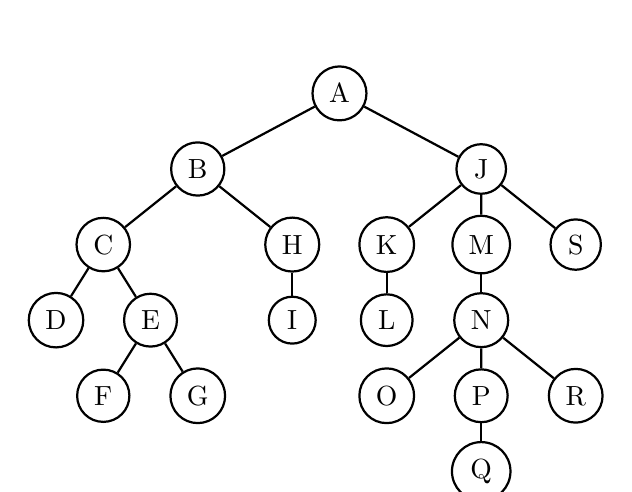
\begin{tikzpicture}
	[thick,scale=0.8, every node/.style={scale=1}]
	\node [circle,draw] {A}
	child {node [circle,draw] {B}
		child {node [circle,draw] {C}
			child {node [circle,draw] {D}}
			child {node [circle,draw] {E}
				child {node [circle,draw] {F}}
				child {node [circle,draw] {G}}
			}
		}
		child [missing] {}
		child {node [circle,draw] {H}
			child {node [circle,draw] {I}}
		}
	}	
	child [missing] {}	
	child [missing] {}	
	child {node [circle,draw] {J}
		child {node [circle,draw] {K}
			child {node [circle,draw] {L}}
		}
		child {node [circle,draw] {M}
			child {node [circle,draw] {N}
				child {node [circle,draw] {O}}
				child {node [circle,draw] {P}
					child {node [circle,draw] {Q}}	
				}
				child {node [circle,draw] {R}}
			}
		}
		child {node [circle,draw] {S}}
	};
	\end{tikzpicture}
	
	\begin{enumerate}[(a)]
		\item What are the leaves? 
		\item What are the children of B? 
		\item What is the depth of G? 
		\item What is the degree of J? 
		\item What are the ancestors of G? 
		\item What are the descendants of G? 
		\item What is the height of the tree? 
		\item What is the degree of the tree? 
		\item Enumerate the nodes in breadth-first order. 
		\item Enumerate the nodes in depth-first preorder. 
		\item Enumerate the nodes in depth-first posterorder. 
	\end{enumerate}
	
	
	%---------------------------------------------------------
	\question{4}{(3') Binary tree property}
	In a rooted tree, the degree of a node is defined as the number of children of the node. For a binary tree, the degree is at least $0$ and at most $2$. We denote $n_0$ to be the number of nodes with degree $0$, $n_1$ to be the number of nodes with degree $1$ and $n_2$ to be the number of nodes with degree $2$. Justify whether $n_0 = n_2 + 1$.\\
	\pagebreak
	
	%---------------------------------------------------------
	\question{5}{(3') Binary Tree Traversal}
	%	Give the preorder, inorder, and postorder traversal of the following tree, where 
	In the lecture, the pre-ordering, post-ordering of tree has been introduced. In fact, for a binary
	tree, the in-ordering of a tree is defined as:
	\begin{enumerate}[(1)]
		\item Check if the current node is empty or null.
		\item Traverse the left subtree by recursively calling the in-order function.
		\item Output the data part of the root (or current node).
		\item Traverse the right subtree by recursively calling the in-order function.
	\end{enumerate}
	
	\begin{figure}[htpb]
		\centering %使插入的图片居中显示
		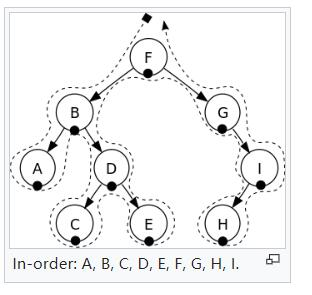
\includegraphics[width=0.4\textwidth]{in_order.jpg}
		\caption{An illustration of an in-ordering of a binary tree}
	\end{figure}
	
	%	\textbf{Tips}:
	%	\begin{enumerate}[(1)]
	%	\item Any node in a tree T, together with all the nodes below it, comprise a \textbf{subtree} of T.
	%	\item A tree whose elements have at most 2 children is called a \textbf{binary tree}. Since each element in a binary tree can have only 2 children, we typically name them the left and right child. The corresponding subtree called
	%	left subtree and right subtree.
	%	\end{enumerate}
	
	
	
	Given the pre-ordering and in-ordering of a binary tree as follows, is it possible to reconstruct the original tree? If it is, write down that tree. If it does not, write NO and enjoy your national holiday.
	
	\begin{enumerate}[(1)]
		\item Pre-ordering: abdeijfcgh
		\item In-ordering: dijefbghca
	\end{enumerate}
	
\end{document}